\documentclass{article}
\usepackage[utf8]{inputenc}
\usepackage{subfig}
\usepackage{amsmath}

\usepackage{graphicx}
\usepackage[legalpaper, portrait, margin=0.5cm]{geometry}

\thispagestyle{empty}
% \renewcommand{\thesubfigure}{\roman{subfigure}}
\begin{document}

\begin{figure}[h]
        \centering
        \subfloat[fully-coherent]{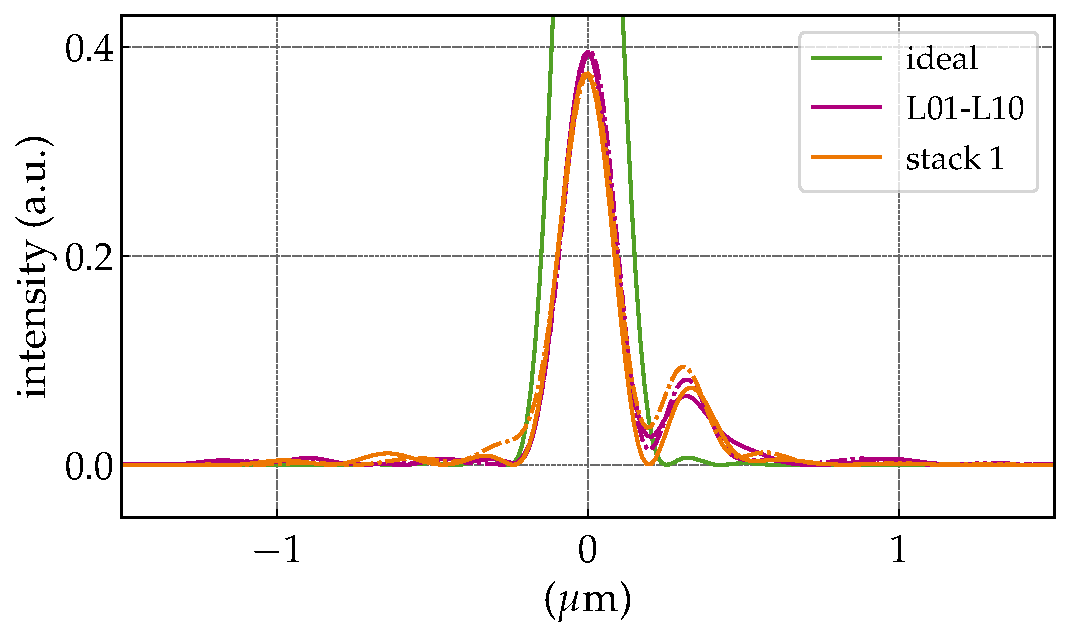
\includegraphics[height=4cm]{figures/ch05/CDn_vs_CDnStack/Strehl_SE_CDn_vs_CDnStack_N.pdf}}\hspace{0.1cm}
        \subfloat[partially-coherent]{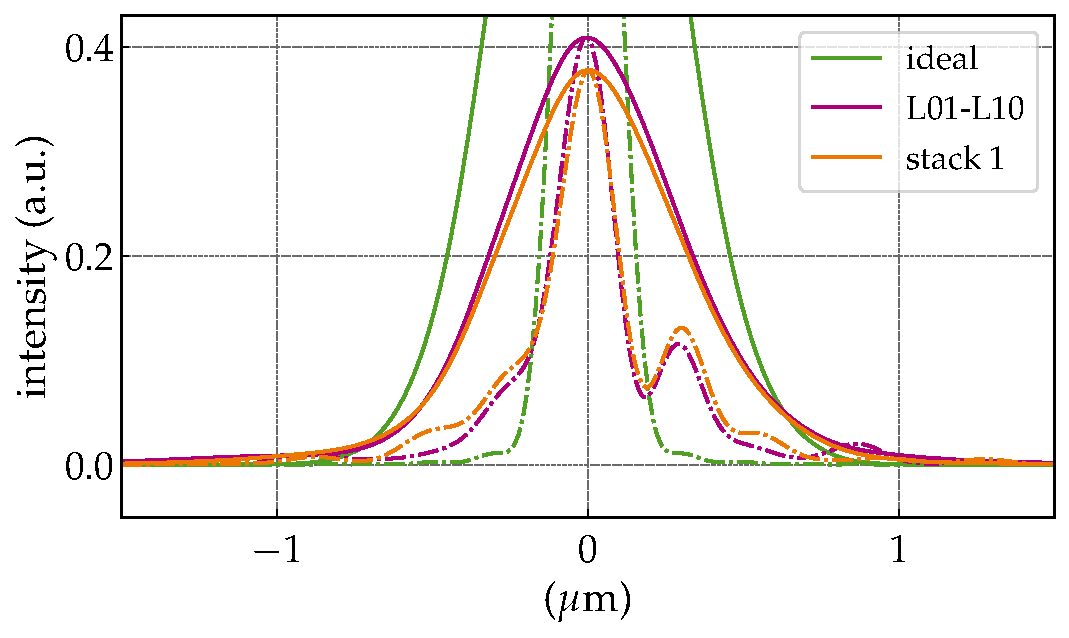
\includegraphics[height=4cm]{figures/ch05/CDn_vs_CDnStack/Strehl_ME_CDn_vs_CDnStack_N.pdf}}
        \caption*{L01-L10 vs. stack 1}
        \subfloat[fully-coherent]{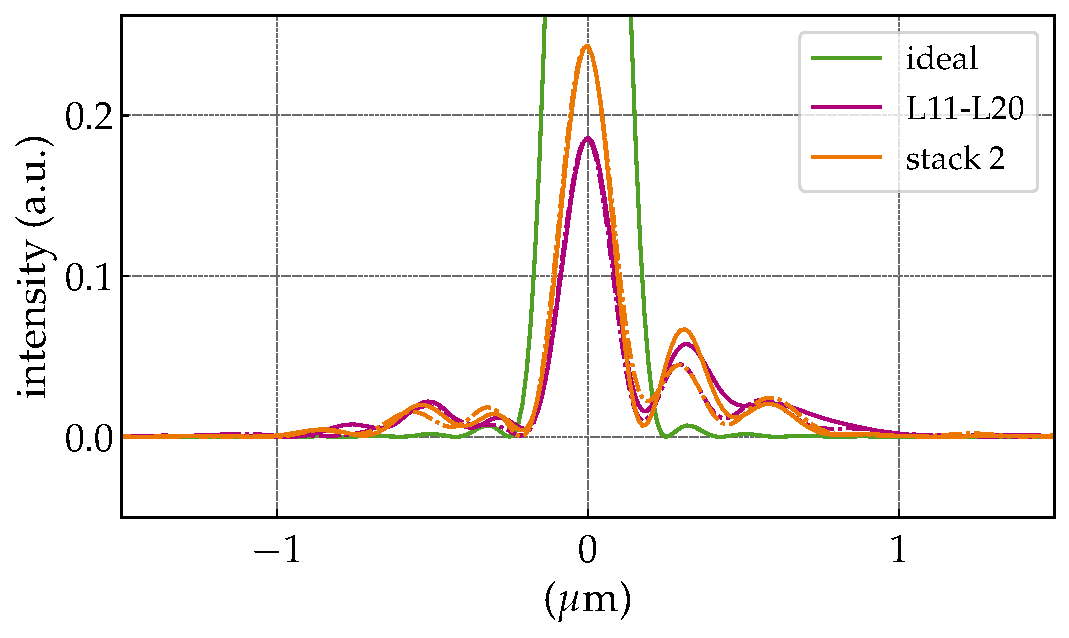
\includegraphics[height=4cm]{figures/ch05/CDn_vs_CDnStack/Strehl_SE_CDo_vs_CDnStack_N.pdf}}\hspace{0.1cm}
        \subfloat[partially-coherent]{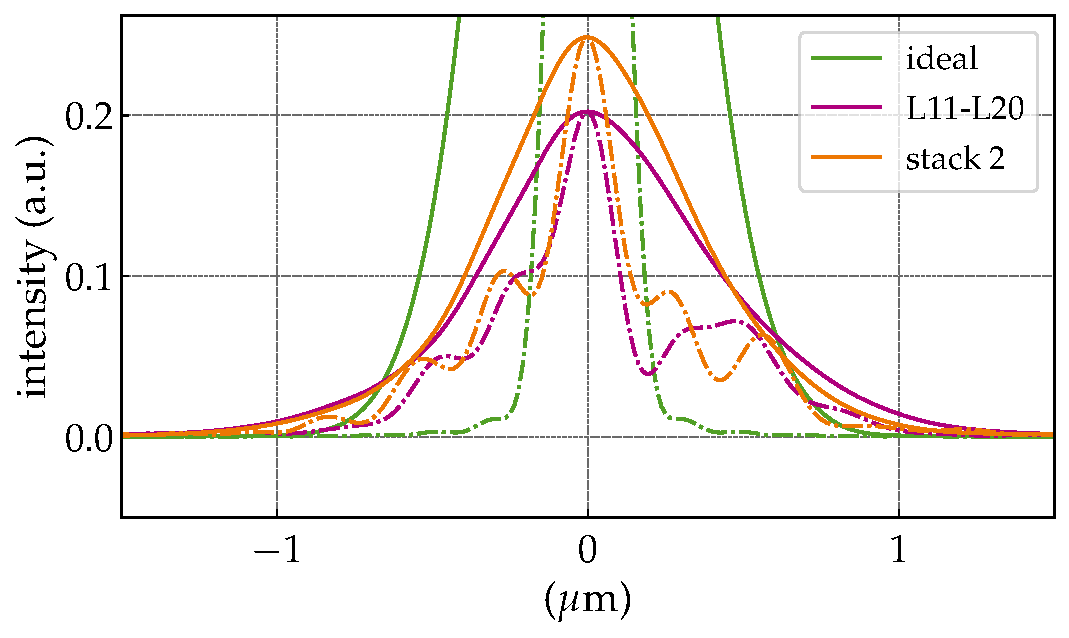
\includegraphics[height=4cm]{figures/ch05/CDn_vs_CDnStack/Strehl_ME_CDo_vs_CDoStack_N.pdf}}
        \caption*{L11-L20 vs. stack 2}
\end{figure}
\end{document}